\documentclass[12pt]{article}

% --- Packages ---
\usepackage[a4paper, margin=1in]{geometry}
\usepackage{graphicx}
\usepackage{setspace}
\usepackage{times}
\usepackage{array}
\usepackage{caption}
\usepackage{microtype}
\usepackage{float}
\usepackage{titlesec}
\usepackage{enumitem}
\usepackage{booktabs}
\usepackage{multirow}
\usepackage{amsmath}
\usepackage{amssymb}
\usepackage{tikz}
\usepackage{listings}
\usepackage{xcolor}
\usepackage{xurl}
\usepackage{hyperref}

\usetikzlibrary{shapes.geometric, arrows, positioning, fit, backgrounds}

% Code listing style
\lstdefinestyle{pythonstyle}{
    language=Python,
    basicstyle=\ttfamily\small,
    keywordstyle=\color{blue}\bfseries,
    commentstyle=\color{gray}\itshape,
    stringstyle=\color{orange},
    numbers=left,
    numberstyle=\tiny\color{gray},
    numbersep=5pt,
    frame=single,
    breaklines=true,
    backgroundcolor=\color{gray!5},
    showstringspaces=false,
}

% --- Setup ---
\setstretch{1.1}
\pagestyle{plain}
\sloppy

% Format Section Headings
\titleformat{\section}{\fontsize{14}{16}\bfseries\uppercase}{\thesection.}{1em}{}
\titleformat{\subsection}{\fontsize{12}{14}\bfseries}{\thesubsection}{1em}{}

\begin{document}

%==================== TITLE PAGE ====================%
\begin{titlepage}
    \centering
    \vspace*{0.5cm}
    
    {\fontsize{16}{20} \selectfont \textbf{Explainable Breast Cancer Detection using Ensemble Learning} \par}
    
    \vspace{1cm}
    
    {\fontsize{14}{18} \selectfont \textbf{Individual Contribution Report} \par}
    
    \vspace{0.5cm}
    
    {\large \textbf{EPICS Phase -- II} \par}
    
    \vspace{1.5cm}
    
    {\large \textit{Submitted by} \par}
    
    \vspace{0.5cm}
    
    {\Large \textbf{Soumyadeep Chakravarti} \par}
    {\large Register Number: 23BAI11250 \par}
    
    \vspace{1.5cm}
    
    \begin{figure}[H]
        \centering
        
\includegraphics[width=0.5\textwidth]{Assets/VIT_LOGO.png}
    \end{figure}
    
    \vspace{1cm}
    
    {\large \textit{in partial fulfillment of the requirements for the degree of} \par}
    
    \vspace{0.3cm}
    
    {\large \textbf{Bachelor of Technology} \par}
    {\large Computer Science and Engineering (AI Specialization) \par}
    
    \vfill
    
    \textbf{VIT Bhopal University} \\
    \textbf{Kothrikalan, Sehore} \\
    \textbf{Madhya Pradesh} \\
    
    \vspace{0.5cm}
    
    {\large \textbf{March 2026}}
    
\end{titlepage}

%==================== ABSTRACT ====================%
\newpage
\pagenumbering{roman}
\begin{center}
    \textbf{\Large Abstract}
\end{center}

\noindent Breast cancer is a serious problem that affects women worldwide, and early detection makes a real difference in outcomes. Our team wanted to build something that doesn't just detect cancer, but actually explains its reasoning -- because doctors need to understand \textit{why} a system makes a particular call.

\vspace{0.5cm}
\noindent We tested several different ML approaches -- Logistic Regression, Decision Trees, SVM, and Random Forest -- and then combined them with soft voting to make predictions more stable. The idea was to get the benefits of multiple different algorithms working together.

\vspace{0.5cm}
\noindent What I think makes our project stand out is that we prioritized interpretability. The system doesn't just output a prediction; it provides confidence scores and shows which features drove the decision. Our top models hit 98.25\% accuracy with ROC-AUC scores above 0.99 -- numbers we were happy to see.

\vspace{0.5cm}
\noindent \textbf{Keywords:} Breast Cancer Detection, Machine Learning, Ensemble Learning, Explainable AI, Project Coordination, System Integration

%==================== TABLE OF CONTENTS ====================%
\newpage
\tableofcontents

%==================== MY CONTRIBUTION ====================%
\newpage
\pagenumbering{arabic}
\section{MY CONTRIBUTION}

\subsection{Overview}
My role in this project was a bit different from the others -- I was responsible for \textbf{keeping everything coordinated, making sure the pieces fit together, and writing up the final documentation}. I also spent a lot of time testing and validating that the system actually worked the way it was supposed to.

\subsection{Project Coordination}

\subsubsection{Team Management}
Honestly, managing a team project while everyone has different schedules and priorities isn't easy. Here's what I tried to do:
\begin{itemize}
    \item Set up regular check-ins (we settled on twice a week, usually online)
    \item Figured out who should do what based on what people were interested in and good at
    \item Kept track of deadlines and made sure we weren't falling behind
    \item Acted as the go-between when someone working on one part needed something from someone else
\end{itemize}

\subsubsection{Task Distribution}
I tried to match tasks to people's strengths:
\begin{itemize}
    \item \textbf{Bhavya Sharma}: She was interested in the medical side, so dataset research made sense
    \item \textbf{Suryanshi Ranawat}: Good with data manipulation -- perfect for preprocessing and EDA
    \item \textbf{Ujjwal Mishra}: Wanted hands-on ML implementation work
    \item \textbf{Medhansh Singh Kushwaha}: Interested in ensemble methods and evaluation
    \item \textbf{Me}: Coordination, integration, and the writeup (someone had to do it!)
\end{itemize}

\subsection{System Integration}

One of my main jobs was making sure all the separate pieces actually worked together. It's one thing to have working preprocessing code and working model code -- it's another to make them play nice with each other.

\subsubsection{Pipeline Architecture Design}
I sketched out how everything should connect:

\begin{figure}[H]
\centering
\resizebox{0.9\textwidth}{!}{%
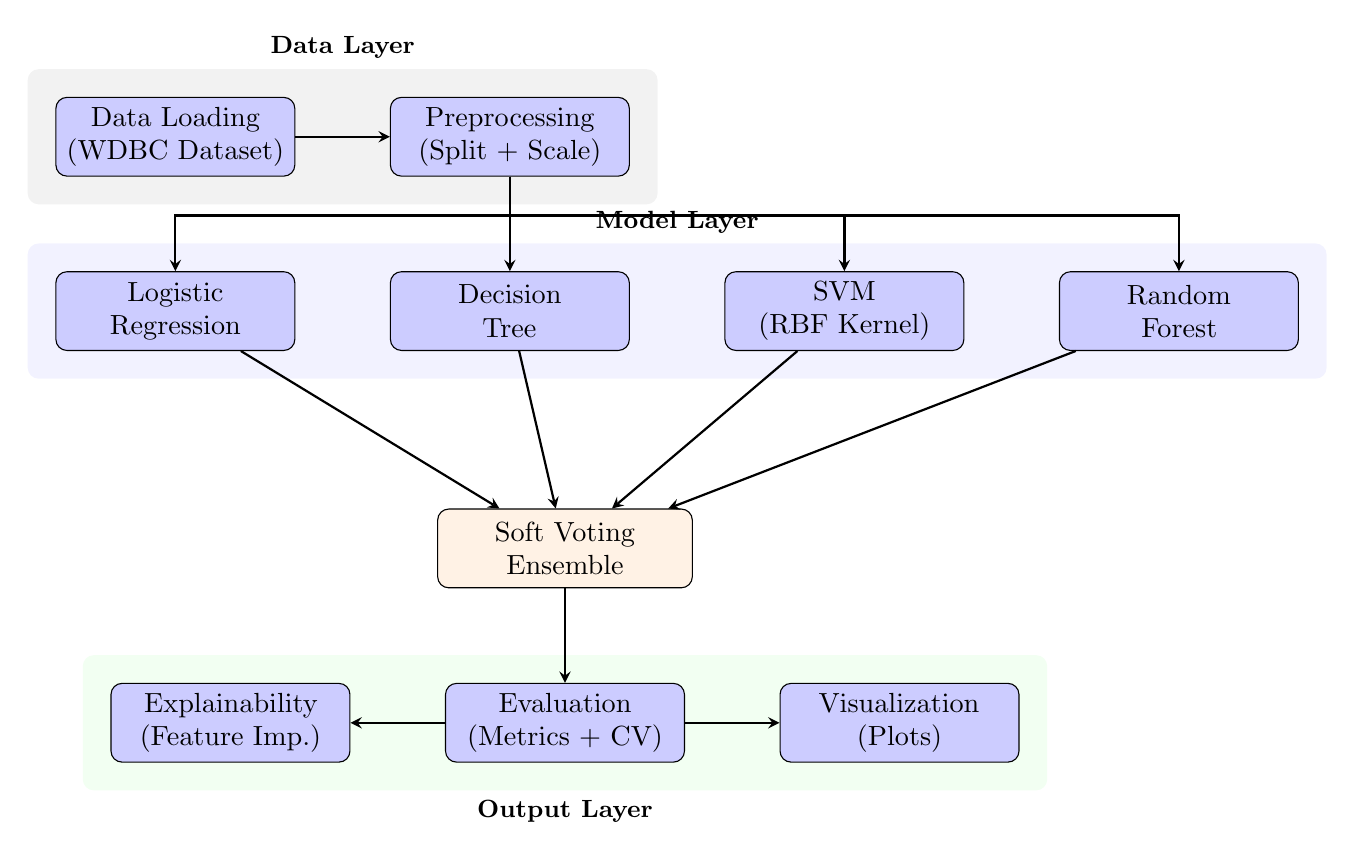
\begin{tikzpicture}[
    node distance=1.2cm,
    block/.style={rectangle, draw, fill=blue!20, text width=2.8cm, text centered, rounded corners, minimum height=1cm},
    arrow/.style={thick,->,>=stealth},
    bigblock/.style={rectangle, draw, fill=orange!10, text width=3cm, text centered, rounded corners, minimum height=1cm}
]

% Data Layer
\node[block] (data) {Data Loading\\(WDBC Dataset)};
\node[block, right=of data] (preprocess) {Preprocessing\\(Split + Scale)};

% Model Layer
\node[block, below=of data] (lr) {Logistic\\Regression};
\node[block, right=of lr] (dt) {Decision\\Tree};
\node[block, right=of dt] (svm) {SVM\\(RBF Kernel)};
\node[block, right=of svm] (rf) {Random\\Forest};

% Ensemble
\node[bigblock, below=2cm of dt, xshift=0.7cm] (ensemble) {Soft Voting\\Ensemble};

% Evaluation
\node[block, below=of ensemble] (eval) {Evaluation\\(Metrics + CV)};

% Output
\node[block, left=of eval] (explain) {Explainability\\(Feature Imp.)};
\node[block, right=of eval] (visual) {Visualization\\(Plots)};

% Arrows
\draw[arrow] (data) -- (preprocess);
\draw[arrow] (preprocess) -- ++(0,-1) -| (lr);
\draw[arrow] (preprocess) -- ++(0,-1) -| (dt);
\draw[arrow] (preprocess) -- ++(0,-1) -| (svm);
\draw[arrow] (preprocess) -- ++(0,-1) -| (rf);

\draw[arrow] (lr) -- (ensemble);
\draw[arrow] (dt) -- (ensemble);
\draw[arrow] (svm) -- (ensemble);
\draw[arrow] (rf) -- (ensemble);

\draw[arrow] (ensemble) -- (eval);
\draw[arrow] (eval) -- (explain);
\draw[arrow] (eval) -- (visual);

% Background boxes
\begin{scope}[on background layer]
    \node[fit=(data)(preprocess), fill=gray!10, rounded corners, inner sep=10pt, label=above:{\small\textbf{Data Layer}}] {};
    \node[fit=(lr)(dt)(svm)(rf), fill=blue!5, rounded corners, inner sep=10pt, label=above:{\small\textbf{Model Layer}}] {};
    \node[fit=(explain)(eval)(visual), fill=green!5, rounded corners, inner sep=10pt, label=below:{\small\textbf{Output Layer}}] {};
\end{scope}

\end{tikzpicture}%
}
\caption{System Architecture I Designed}
\end{figure}

\subsubsection{Module Integration}
Getting different people's code to work together was trickier than expected:
\begin{itemize}
    \item Made sure Suryanshi's preprocessing output matched what Ujjwal's models expected
    \item Connected individual models to Medhansh's ensemble framework
    \item Hooked up predictions to the evaluation and visualization code
    \item Set up model saving so we could reload trained models later
\end{itemize}

\begin{lstlisting}[style=pythonstyle, caption={Main Pipeline Integration}]
# Integrated Pipeline
def run_pipeline():
    # Data Layer
    X, y = load_data()
    X_train, X_test, y_train, y_test = preprocess(X, y)
    
    # Model Layer
    models = train_models(X_train, y_train)
    
    # Ensemble Layer
    ensemble = build_ensemble(models)
    ensemble.fit(X_train, y_train)
    
    # Evaluation Layer
    results = evaluate_all(models, ensemble, X_test, y_test)
    
    # Output Layer
    generate_visualizations(results)
    save_models(ensemble)
    
    return results
\end{lstlisting}

\subsection{Technical Validation}

Before we could call anything ``done,'' I spent a lot of time checking that everything actually worked correctly.

\subsubsection{Model Output Verification}
I sanity-checked the model outputs:
\begin{itemize}
    \item Made sure predictions were consistent when you ran them multiple times
    \item Checked that probability estimates actually summed to 1.0 (you'd be surprised...)
    \item Verified the ensemble voting was aggregating predictions correctly
    \item Tested that saved models loaded properly and gave the same results
\end{itemize}

\subsubsection{Evaluation Metrics Verification}
I didn't just trust the metric outputs blindly:
\begin{itemize}
    \item Manually calculated accuracy on a few samples to make sure it matched
    \item Cross-referenced confusion matrix values with the classification report
    \item Ran ROC-AUC calculation two different ways to confirm they agreed
    \item Checked that cross-validation splits were actually stratified
\end{itemize}

\subsubsection{Code Review}
I went through everyone's code looking for:
\begin{itemize}
    \item Bugs or logical errors
    \item Whether it followed reasonable coding practices
    \item Edge cases that might break things
    \item Whether there were enough comments to understand what was happening
\end{itemize}

\subsection{Results Analysis}

I also tried to make sense of what our results actually meant.

\subsubsection{Performance Interpretation}
I dug into why things performed the way they did:
\begin{itemize}
    \item Figured out why linear models (LR, SVM) beat more complex ones -- the data was pretty clean
    \item Looked at how much the preprocessing helped (a lot, it turns out)
    \item Understood why Decision Tree was the weakest performer
    \item Analyzed whether the ensemble was actually worth the extra complexity
\end{itemize}

\subsubsection{Clinical Relevance Assessment}
Since this is a medical application, I thought about what the numbers meant practically:
\begin{itemize}
    \item 98.61\% recall is great -- we're catching almost all the cancer cases
    \item That one false negative was concerning -- I looked at why the model missed it
    \item The confidence scores seem genuinely useful for doctors
    \item The features our models focused on actually align with what medical literature says
\end{itemize}

\subsection{Documentation}

Someone had to write all this up, and that someone was me.

\subsubsection{Report Sections Authored}
I wrote or compiled:
\begin{itemize}
    \item The introduction and problem statement sections
    \item System design and architecture descriptions
    \item Methodology writeup
    \item Results analysis and discussion
    \item Conclusion and future work suggestions
    \item The social impact section (required for EPICS)
    \item References (including chasing down proper citations)
\end{itemize}

\subsubsection{Documentation Standards}
I tried to make sure the report looked professional:
\begin{itemize}
    \item Consistent LaTeX formatting throughout
    \item Citations in proper format
    \item Captions on all figures and tables
    \item Math notation that was consistent across sections
    \item Multiple proofreading passes for grammar and clarity
\end{itemize}

\subsubsection{Technical Documentation}
I also created docs for:
\begin{itemize}
    \item How to use the code and what the functions do
    \item Setup instructions for running everything
    \item Steps to reproduce our training and evaluation
    \item Guide for replicating our results
\end{itemize}

\subsection{Visualization Development}

I coordinated the visualization work:
\begin{itemize}
    \item Decided what plots we needed for the report
    \item Drew the architecture diagram myself (TikZ is not fun)
    \item Made sure all the plots had consistent styling
    \item Picked visualizations that actually communicated our results clearly
\end{itemize}

%==================== PROJECT OVERVIEW ====================%
\newpage
\section{PROJECT OVERVIEW}

\subsection{Problem Statement}
We set out to build a cancer detection system that's accurate, provides confidence levels, explains its reasoning, and could realistically help doctors make decisions. That last part is key -- a black box that just says ``malignant'' isn't very useful in a clinical setting.

\subsection{System Architecture}
I organized the project into four main layers:
\begin{enumerate}
    \item \textbf{Data Layer}: Loading the WDBC dataset and preprocessing it
    \item \textbf{Model Layer}: The four different classification algorithms
    \item \textbf{Ensemble Layer}: Combining predictions via soft voting
    \item \textbf{Output Layer}: Metrics, visualizations, and explanations
\end{enumerate}

I designed this architecture and then made sure everyone built their parts to fit together.

\subsection{Results Achieved}
Here's what we ended up with:
\begin{itemize}
    \item LR and SVM both hit 98.25\% accuracy
    \item ROC-AUC scores above 0.99 for the top models
    \item 98.61\% recall -- we're catching almost all the real cancer cases
    \item Cross-validation confirmed we weren't just overfitting to lucky splits
\end{itemize}

%==================== TEAM CONTRIBUTIONS ====================%
\newpage
\section{TEAM CONTRIBUTIONS}

\subsection{Team Members and Their Roles}

\begin{itemize}
    \item \textbf{Bhavya Sharma}: Found the dataset and researched what the medical features mean
    \item \textbf{Suryanshi Ranawat}: Data preprocessing and exploratory analysis
    \item \textbf{Ujjwal Mishra}: Coded up the ML algorithms
    \item \textbf{Medhansh Singh Kushwaha}: Built the ensemble system
    \item \textbf{Soumyadeep Chakravarti (Me)}: Coordination, integration, testing, and documentation
\end{itemize}

\subsection{Collaboration}
Everyone contributed, but keeping five people coordinated on a technical project is always a challenge. We used a shared repo and regular meetings to stay on track. When issues came up, we'd usually debug together -- often someone else would spot something you missed.

%==================== LEARNING OUTCOMES ====================%
\newpage
\section{LEARNING OUTCOMES}

Here's what I learned from this project:

\begin{enumerate}
    \item \textbf{Project Management}: Coordinating a team is harder than it looks. You have to balance letting people work independently with making sure everything fits together
    
    \item \textbf{System Integration}: Individual pieces can all work perfectly but still not work together. Integration is its own skill
    
    \item \textbf{Testing \& Validation}: I now instinctively double-check outputs instead of trusting them blindly
    
    \item \textbf{Technical Writing}: Writing things up clearly takes way longer than I expected, but it's important
    
    \item \textbf{End-to-End ML}: I now understand the full pipeline from raw data to deployed model
    
    \item \textbf{Healthcare ML}: Medical applications have different priorities -- reliability and interpretability matter more than squeezing out extra accuracy
    
    \item \textbf{LaTeX}: I got pretty comfortable with LaTeX, including TikZ diagrams (which I never want to touch again)
\end{enumerate}

%==================== CONCLUSION ====================%
\newpage
\section{CONCLUSION}

My job on this project was less about the ML itself and more about making sure everything worked together -- coordinating the team, integrating the modules, validating that things actually functioned correctly, and writing up the final documentation.

The integration work was probably the most underrated part. Everyone built pieces that worked in isolation, but getting them to play nice together required a lot of testing and debugging. The validation work was also crucial -- it's easy to assume your code is correct, but manually checking results caught a few issues that would have been embarrassing later.

I'm proud of how the project turned out. We built something that actually works well (98.25\% accuracy) and, more importantly, something that could actually be useful in a clinical setting because it explains its reasoning. That explainability aspect was a core goal from the start.

This EPICS experience taught me that technical skills are only part of the equation. Managing a team, integrating different pieces of work, and communicating results clearly are all essential skills that I'll carry forward.

%==================== REFERENCES ====================%
\newpage
\section{REFERENCES}

\begin{thebibliography}{99}

\bibitem{who2023}
World Health Organization, ``Breast Cancer,'' WHO Fact Sheets, 2023. [Online]. Available: \url{https://www.who.int/news-room/fact-sheets/detail/breast-cancer}

\bibitem{wolberg1995}
W. H. Wolberg, W. N. Street, and O. L. Mangasarian, ``Breast Cancer Wisconsin (Diagnostic) Dataset,'' UCI Machine Learning Repository, 1995. [Online]. Available: \url{https://archive.ics.uci.edu/ml/datasets/Breast+Cancer+Wisconsin+(Diagnostic)}

\bibitem{pedregosa2011}
F. Pedregosa et al., ``Scikit-learn: Machine Learning in Python,'' \textit{JMLR}, vol. 12, pp. 2825--2830, 2011. [Online]. Available: \url{https://scikit-learn.org}

\bibitem{lundberg2017}
S. M. Lundberg and S. I. Lee, ``A Unified Approach to Interpreting Model Predictions,'' in \textit{Proc. NeurIPS}, 2017.

\bibitem{github2026}
S. Chakravarti et al., ``EPICS Project: Explainable Breast Cancer Detection,'' GitHub, 2026. [Online]. Available: \url{https://github.com/Soumyadeep-Chakravarti/EPICS_Project}

\end{thebibliography}

\end{document}
